\documentclass[a4paper,11pt]{article}
\usepackage[utf8]{inputenc}
\usepackage[T1]{fontenc}
\usepackage[french]{babel}
\usepackage[right=2.5cm, left=2.5cm, bottom=4cm, top=3cm]{geometry}
\usepackage{textcomp}
\usepackage{graphicx}
\usepackage{mathtools,amssymb,amsthm}
\usepackage{lmodern}
\usepackage{multirow}
\usepackage{array}
\usepackage{longtable}

\title{\vspace{13em}{\huge Manuel utilisateur}}
\author{Clément Caumes - Mehdi Merimi - Sarah Ngoc-Mai Pho - Maxime Gonthier\\
		\vspace{2em}\\
		JNotes
		\vspace{2em}}

\begin{document}
	
	\pagenumbering{gobble}\clearpage
	\maketitle\vspace{13em}
\newpage
\tableofcontents
\newpage\clearpage\pagenumbering{arabic}
	
	\section{Introduction}
		L'application "JNotes" est un outil permettant la gestion de notes utilisant asciidoctor.\\
		Elle permet à l'utilisateur de modifier, supprimer, lister ou voir des notes. Elle contient également une fonction de recherche et un index triant les notes par ordre alphabétique.
		Ce guide a été conçu pour faciliter l'utilisation de l'application.
			
	\section{Fonctionnalitées}
		\subsection{Lancement de l'application}
		\begin{itemize}
				\item $mvn test$ lance l'ensemble des tests junit.\\
				\\
				\centerline{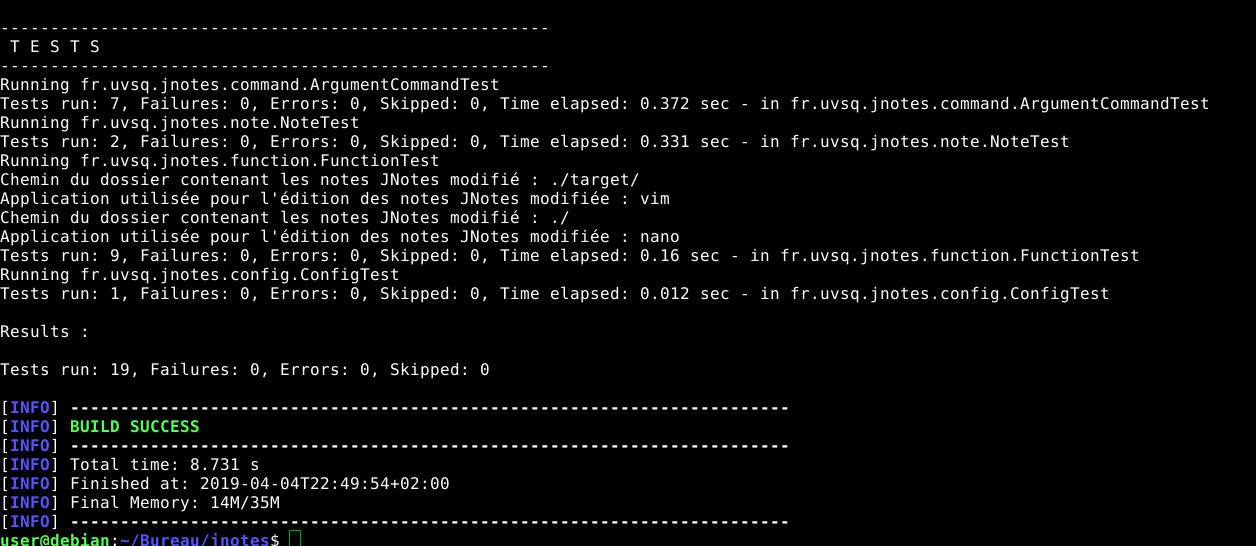
\includegraphics[scale=0.4]{Captures/test.png}}
				\\
				\item $mvn package$ compile le projet et lance les tests.\\
				\\
				\centerline{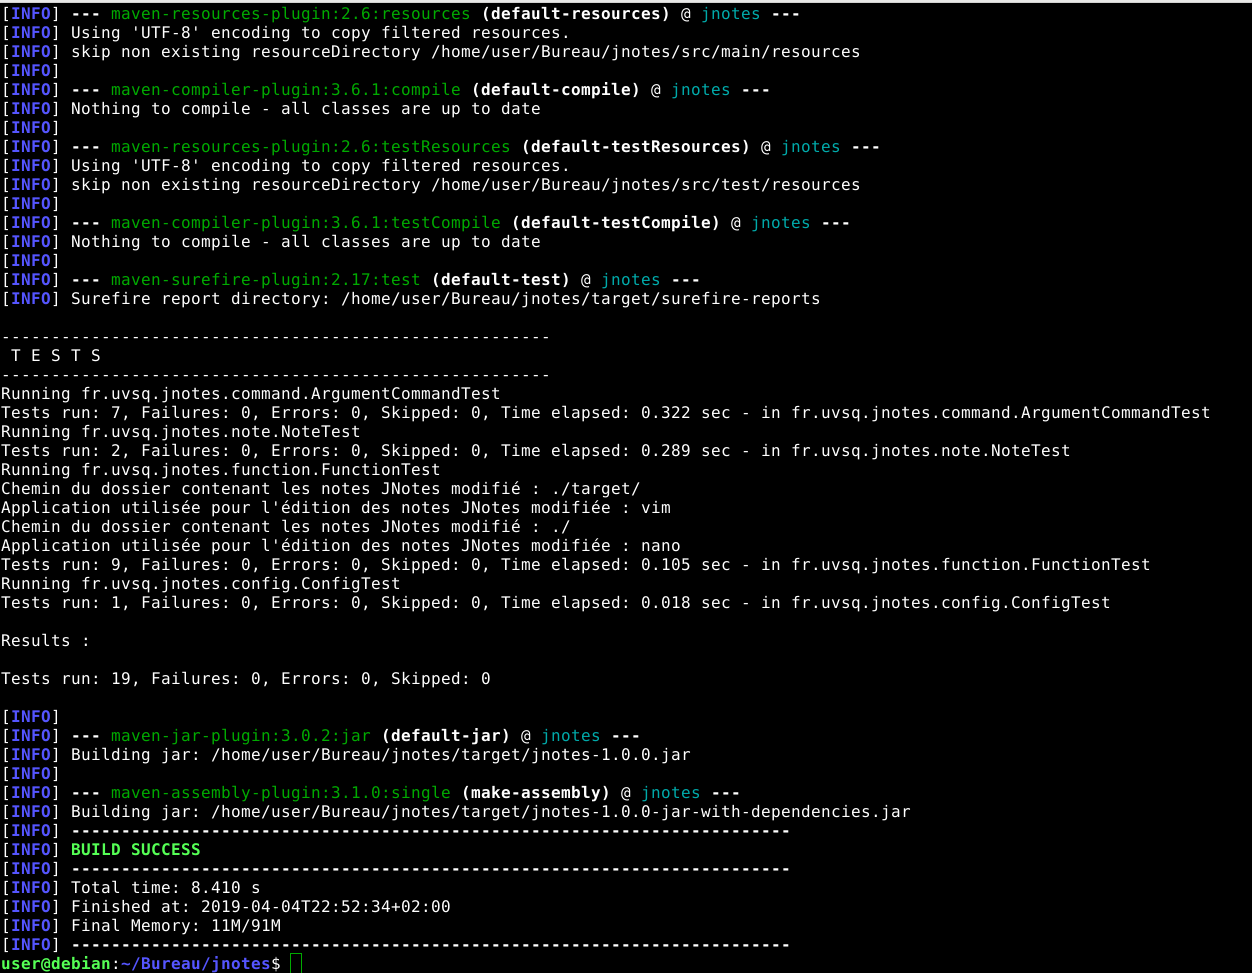
\includegraphics[scale=0.4]{Captures/mvnpackage.png}}
				\\
				\item $java -jar target/jnotes-1.0.0-jar-with-dependencies.jar $ execute le programme.\\
				\\
				\centerline{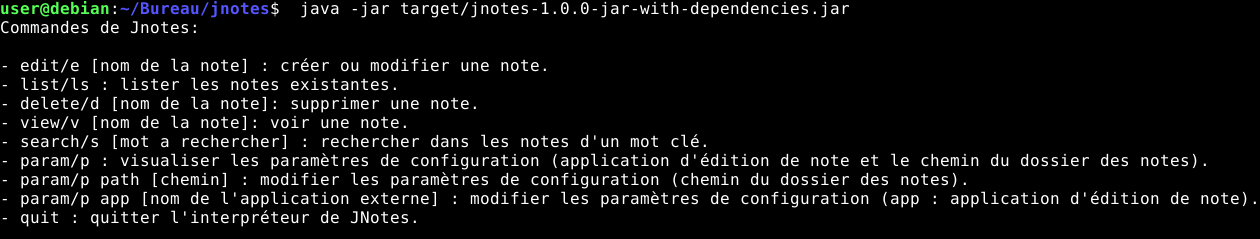
\includegraphics[scale=0.4]{Captures/ecranacceuil.png}}
				\\
			\end{itemize}
		Une fois l'application lancé l'utilisateurs a acces à différentes fonctionnalitées décrite si dessous.
		\subsection{Edit}
			En tapant edit [nom de la note] ou e [nom de la note] un écran apparait affichant la note.
			Si la note n'existait pas elle est créer et pré remplis.\\
			\\
			\centerline{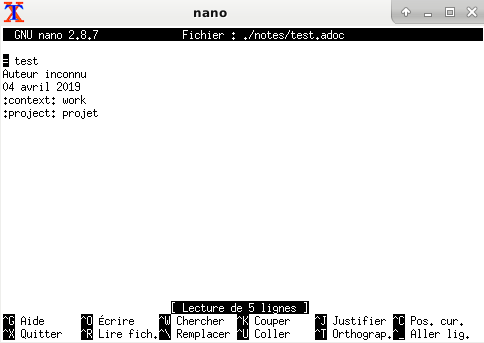
\includegraphics[scale=0.9]{Captures/edit.png}}
			\\
		\subsection{Liste}
			En tapant list ou ls, le terminal affiche la liste des notes existantes\\
			\\
			\centerline{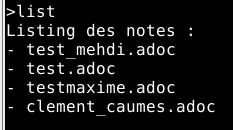
\includegraphics[scale=0.9]{Captures/list.png}}
			\\
		\subsection{Delete}
			En tapant delete [nom de la note] ou d [nom de la note] le programme supprime la note et affiche un message.\\
			\\
			\centerline{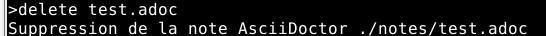
\includegraphics[scale=0.9]{Captures/delete.png}}
			\\
		\subsection{View}
			En tapant view [nom de la note] ou v [nom de la note] la note est ouverte dans firefox.\\
			\\
			\centerline{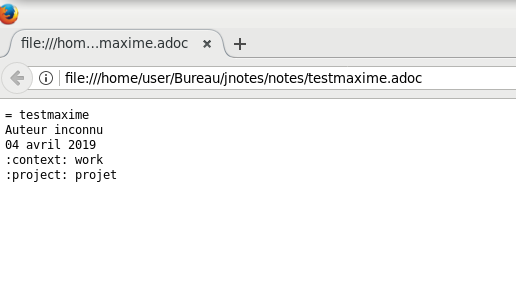
\includegraphics[scale=0.9]{Captures/view.png}}
			\\
		\subsection{Search}
			A ecrire
			\\
			%~ \centerline{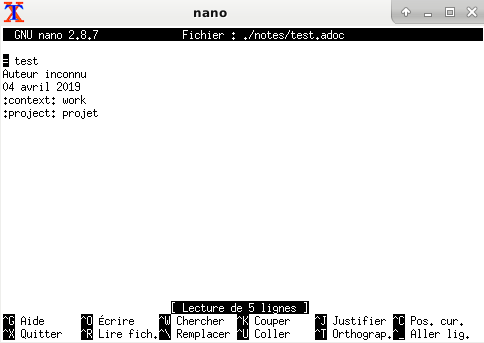
\includegraphics[scale=0.9]{Captures/edit.png}}
			\\
		\subsection{Param}
			En tapant param ou p, le terminal affiche les paramètres, c'ets à dire l'application d'édition des notes et le chemin du dossier contenant les notes.\\
			\\
			\centerline{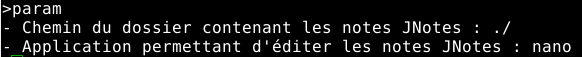
\includegraphics[scale=0.9]{Captures/param.png}}
			\\	
		\subsection{Param path}
			En tapant param path [nouveau chemin] ou p path [nouveau chemin], le chemin du dossier contenant les notes est modifié.\\
			\\
			\centerline{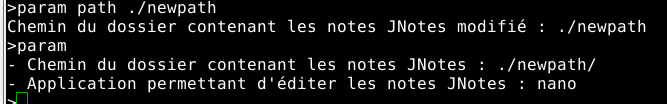
\includegraphics[scale=0.6]{Captures/parampath.png}}
			\\	
		\subsection{Param app}
			En tapant param app [nom de l'application] ou p app [nom de l'application], l'application de modification des notes est modifié.\\
			\\
			\centerline{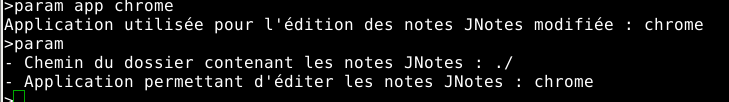
\includegraphics[scale=0.6]{Captures/paramapp.png}}
			\\	
		\subsection{Quit}
			Taper quit permet de quitter l'application.
		
	
\end{document}
